\documentclass{beamer}

\mode<presentation>
{
  %\usetheme{CambridgeUS}
  \usefonttheme{professionalfonts}

  \usetheme{Singapore}
  \usecolortheme{orchid}
  %\setbeamercovered{transparent}
}

\usepackage{pgfpages}

\usepackage{verbatim,fancyvrb,times}
\usepackage{bm}
\usepackage[english]{babel}
\usepackage[utf8]{inputenc}
\usefonttheme[onlymath]{serif}
\usepackage[T1]{fontenc}
% Or whatever. Note that the encoding and the font should match. If T1
% does not look nice, try deleting the line with the fontenc.

\usepackage{amsmath}
\usepackage[amssymb]{SIunits}

\usepackage{hyperref}

\usepackage{tikz}
\usetikzlibrary{shapes,arrows,decorations.pathmorphing,calc}

\usetikzlibrary{shadows}
\definecolor{uaf red}{HTML}{E41A1C}
\definecolor{uaf blue}{HTML}{377EB8}
\definecolor{uaf green}{HTML}{4DAF4A}
\definecolor{uaf violet}{HTML}{984EA3}
\definecolor{uaf orange}{HTML}{FF7F00}
\setbeamercolor{boxed}{fg=black,bg=uaf yellow}

\newenvironment{transbox}{%

\begin{tikzpicture}
\node[drop shadow,rounded corners,text width=0.9\textwidth,fill=uaf violet, fill opacity=0.5,text opacity=1] \bgroup
}{
\egroup;\end{tikzpicture}} 

\newcommand{\Div}{\nabla\cdot}
\newcommand{\eps}{\epsilon}
\newcommand{\grad}{\nabla}
\newcommand{\lap}{\triangle}
\DeclareMathOperator{\trace}{tr}
\renewcommand{\bar}{\overline}

\newcommand{\ddx}[1]{\frac{\partial #1}{\partial x}}
\newcommand{\ddy}[1]{\frac{\partial #1}{\partial y}}

\newcommand {\jl}{[\![}
\newcommand {\jr}{]\!\hskip 0.003cm ]}
\newcommand{\bpsi}{\boldsymbol{\psi}}
\newcommand{\bPsi}{\boldsymbol{\Psi}}
\newcommand{\bphi}{\boldsymbol{\phi}}
\newcommand{\bPhi}{\boldsymbol{\Phi}}
\newcommand{\bn}{\mathbf{n}}
\newcommand{\bq}{\mathbf{q}}
\newcommand{\bv}{\mathbf{v}}
\newcommand{\D}{\,\mathrm{d}}
\newcommand{\Tsnow}{T_{\text{snow}}}


%\setbeamercolor{redtext}{fg=red!80!black}
\setbeamercolor{redtext}{fg=red!94!black}
%\setbeamercolor{greentext}{fg=green!80!black}
\setbeamercolor{greentext}{fg=green!60!black}
%\setbeamercolor{bluetext}{fg=blue!70!black}
\setbeamercolor{bluetext}{fg=blue!90!black}
\setbeamercolor{yellowtext}{fg=yellow!95!black}
\setbeamercolor{orangetext}{fg=yellow!50!red}

\newcommand{\green}{\usebeamercolor[fg]{greentext}}
\newcommand{\blue}{\usebeamercolor[fg]{bluetext}}
\newcommand{\red}{\usebeamercolor[fg]{redtext}}

\renewcommand{\L}{\emph{Left}}
\newcommand{\R}{\emph{Right}}



\title{Should your ice sheet model \\ conserve energy?}

\author{Ed Bueler}

\institute{\tiny Dept of Mathematics and Statistics and Geophysical Institute \\
  University of Alaska Fairbanks}

\date{21 April, 2011}



\setbeamerfont{date}{size=\scriptsize}

%\begin{comment}
\AtBeginSection[]
{
  \begin{frame}<beamer>
    \frametitle{Outline}
    \tableofcontents[currentsection]
  \end{frame}
}
%\end{comment}

\begin{document}
\graphicspath{{figs/}}

\begin{frame}
  \titlepage
\end{frame}

\begin{comment}
\begin{frame}
  \frametitle{Outline}
  \tableofcontents[hideallsubsections]
  % You might wish to add the option [pausesections]
\end{frame}
\end{comment}


\section[ice sheets and models thereof]{what is an ice sheet? \quad what is PISM?}\subsection*{}


\begin{frame}{what is an ice sheet?}
  \begin{figure}
    \includegraphics[width=0.9\textwidth]{ice-sheet-cartoon}\\
    \tiny{(figure modified from ICESat brochure)}
  \end{figure}
\end{frame}


\begin{frame}{``ice sheet'' versus all that other ice}
  \begin{itemize}
    \item an ice sheet is a big glacier
    \item there are two right now: Greenland and Antarctic
    \item flows because of gravity
       \begin{itemize}
       \small
       \item[$\ast$] by deformation mostly ($\exists$ crevasses)
       \normalsize
       \end{itemize}
    \item slow flow \quad $\longleftarrow$ \emph{technical term}!
    \item almost all of an ice sheet is \emph{grounded} and \emph{thick} ($> 200$ m)
      \begin{columns}
      \begin{column}{0.7\textwidth}
      \begin{itemize}
      \small
      \item[$\ast$] versus sea-ice
      \item[$\ast$] \dots which is \emph{floating} and \emph{thin} ($\le 5$ m)  
      \item[$\ast$] ice shelves are thick and floating \emph{and attached to an ice sheet}
      \normalsize
      \end{itemize}
      \end{column}
      \begin{column}{0.2\textwidth}
      \includegraphics[width=\textwidth]{seaice-bad}
      \end{column}
      \end{columns}
  \end{itemize}
\end{frame}


\begin{frame}
  \frametitle{example: Greenland ice sheet}
  
\bigskip\bigskip
\begin{center}
\textsc{[show movie]}
\end{center}
\vfill
\end{frame}


\begin{frame}
  \frametitle{observation: Greenland ice is flowing toward ocean}

\begin{itemize}
\small
\item Greenland central elevation about 3300 m = 10,800 ft a.s.l.
\item ice is about that thick, too; removing it would leave a shallow sea
\item \dots its a ``pile'' of ice which flows outward into the sea
\normalsize
\end{itemize}

\begin{columns}
\begin{column}{0.5\textwidth}
\begin{center}
    \includegraphics[width=0.6\textwidth]{Greenland_usurf}
\end{center}
\end{column}
\begin{column}{0.5\textwidth}
\begin{center}
    %\includegraphics[width=0.65\textwidth]{../GGseminar2011/figures/modis-insar}
    \texttt{../GGseminar2011/figures/modis-insar.png}

    \tiny [InSAR = I.~Joughin; MODIS = M.~Fahnestock]
\end{center}
\end{column}
\end{columns}
\end{frame}


\begin{frame}
  \frametitle{observation: Greenland ice has sped up \\ \dots when blockages are removed}

\begin{columns}
\begin{column}{0.6\textwidth}
\begin{center}
  \includegraphics[width=\textwidth]{Jakobshavn_groundline_retreat}
\end{center}
\end{column}
\begin{column}{0.4\textwidth}
\begin{center}
  \includegraphics[width=\textwidth]{Jakobshavn_speedup}

\bigskip

  %\includegraphics[width=0.5\textwidth]{../GGseminar2011/figures/MODISGreenlandJakobshavn}
  \texttt{../GGseminar2011/figures/MODISGreenlandJakobshavn.png}
\end{center}
\end{column}
\end{columns}
\end{frame}


\begin{frame}
  \frametitle{observations: Greenland is losing mass}

\begin{itemize}
\item Greenland ice sheet mass is $2.7 \times 10^9$ gigatonnes (Gt) % = 2.93466 10^6 km^3  volume, from SeaRISE-Greenland 5km data
\item if \emph{all} melted, = 7 m of sea level rise \dots do not hold breath
\item but observations do show mass is dropping:
\end{itemize}
\medskip

\begin{center}
    \includegraphics[width=0.65\textwidth]{greenlandboxes}
\end{center}
\end{frame}


\begin{frame}
  \frametitle{mathematical/numerical modeling success \\ would look like \emph{this}:}

\vspace{-0.2cm}
\begin{center}
    %\includegraphics[width=0.65\textwidth]{../GGseminar2011/figures/ts_grn_mass_2003-2010_CONST1.pdf}
    \texttt{../GGseminar2011/figures/ts\_grn\_mass\_2003-2010\_CONST1.pdf}
\end{center}

\vspace{-0.4cm}
\begin{itemize}
\small
  \item new result from Aschwanden, Adalgeirsdottir and Khroulev, using HIRHAM+PISM, comparing to gravimetry from GRACE
  \item it is less than the understanding which goes into it
  \item \emph{and} it is less than meets the eye
    \begin{itemize}
    \item[$\ast$] mostly shows surface mass rates are well-modeled
    \end{itemize}
\end{itemize}
\end{frame}


\begin{frame}
  \frametitle{what is an ``ice sheet model''?}
\small

\vspace{-0.4cm}

\begin{itemize}
\item it describes ice as a slow, viscous fluid
\item it cuts the fluid into pieces and approximately solves the PDEs for such fluids (= non-Newtonian Stokes equations)
\item the only body force it includes is gravity \dots there are additional boundary forces from ocean and bedrock
  \begin{columns}
  \begin{column}{0.6\textwidth}
  \begin{itemize}
  \small
  \item[$\ast$] slow = (inertia plays negligible role in Newton's law: ``$F=0$'' instead of ``$F=ma$'')
  \item[$\ast$] \dots therefore geometry and boundary stress and ice strength determine velocity instantaneously
  \normalsize
  \end{itemize}
  \end{column}
  \begin{column}{0.3\textwidth}
  \includegraphics[width=\textwidth]{pancakes}
  \end{column}
  \end{columns}
\end{itemize}
\end{frame}


\begin{frame}
  \frametitle{what is an ``ice sheet model''? 2}
\small

\begin{itemize}
\item model \emph{inputs} at start time: surface elevation, bedrock elevation, ice temperature\footnote{\tiny \dots no one actually can provide this last input \dots}
\item model \emph{boundary inputs}: surface mass and energy rates
  \begin{itemize}
  \item[$\ast$] an ice sheet model ``owns'' ice and bedrock if it runs as part of a general climate/circulation model:
  \end{itemize}
  \begin{center}
  \includegraphics[width=0.7\textwidth]{climate-cartoon}
  \end{center}
\item model \emph{outputs} (at each time): surface elevation, isostacy, velocity, ice temperature, \only<1>{basal melt rate, \alert{age of the ice},}\only<2>{\alert{basal melt rate}, age of the ice,} \alert{rate of total mass change}
\end{itemize}


\end{frame}


\begin{frame}
  \frametitle{Parallel Ice Sheet Model (PISM)}

\begin{itemize}
\item homepage\qquad \texttt{www.pism-docs.org}
\item completely open source: C++ and python
\item well-documented for users and developers
\end{itemize}

\begin{center}
    \includegraphics[width=0.75\textwidth]{pismdocs-page}
\end{center}

\scriptsize
supported by NASA, and now a joint project with PIK in Germany
\end{frame}


\begin{frame}
  \frametitle{PISM developers, then and now}

\tikzstyle{format} = [draw, thin, fill=blue!20]
\tikzstyle{medium} = [ellipse, draw, thin, fill=green!20, font=\footnotesize]

\begin{figure}
\begin{tikzpicture}[node distance=4cm, auto,>=latex', thick]
    % We need to set at bounding box first. Otherwise the diagram
    % will change position for each frame.
    \path[use as bounding box] (-5,-7) rectangle (5,3);
    \path[-]<1> node[format] (old) {$\begin{matrix} \text{Lingle} \\ \text{Bueler} \\ \text{Brown} \end{matrix}$}  node[above of=old, font=\tiny, node distance=1cm] {UAF 2002--2007};
    \path[-]<2> node[format] (earlycore) {$\begin{matrix} \text{Bueler} \\ \text{Khroulev} \end{matrix}$};
    \path[-]<2> node[above of=earlycore, font=\tiny, node distance=0.75cm] {UAF 2008};
    \path[-]<3-> node[format, font=\footnotesize] (core) {$\begin{matrix} \text{Bueler} \\ \text{Khroulev} \\ \text{Aschwanden} \end{matrix}$}  node[above of=core, font=\tiny, node distance=2cm] {2009--};
    \path[-]<3> node[below of=earlycore, node distance=3cm] (photo) {\includegraphics[width=6cm]{group}};
    \path[-]<4-> node[medium, right of=core] (pik) {$\begin{matrix} \text{Levermann} \\ \text{Martin} \\ \text{Winkelmann} \\ \text{Albrechts} \end{matrix}$}  node[above of=pik, font=\tiny, node distance=1.4cm] {PIK} (core) edge node[font=\tiny, text width=1cm] {ice shelves, calving} (pik);
    \path[-]<4-> node[medium, left of=core] (inverse) {$\begin{matrix} \text{Maxwell} \\ \text{Habermann} \\ \text{Truffer} \end{matrix}$}  node[above of=inverse, font=\tiny, node distance=1.3cm] {UAF}
                  (core) edge node[font=\tiny, text width=1cm] {inverse methods} (inverse);
    \path[-]<4-> node[medium, below left of=core] (regional) {DellaGiustina}  node[above of=regional, font=\tiny, node distance=0.5cm] {UAF}
                  (core) edge node[font=\tiny, text width=1cm] {regional model} (regional);
    \path[-]<4-> node[medium, below right of=core] (smb) {Hock} node[above of=smb, font=\tiny, node distance=0.5cm] {UAF}
                  (core) edge node[font=\tiny, text width=1cm] {surface processes} (smb);
\end{tikzpicture}
\end{figure}
\end{frame}


\begin{frame}
  \frametitle{PISM major users}

\begin{center}
    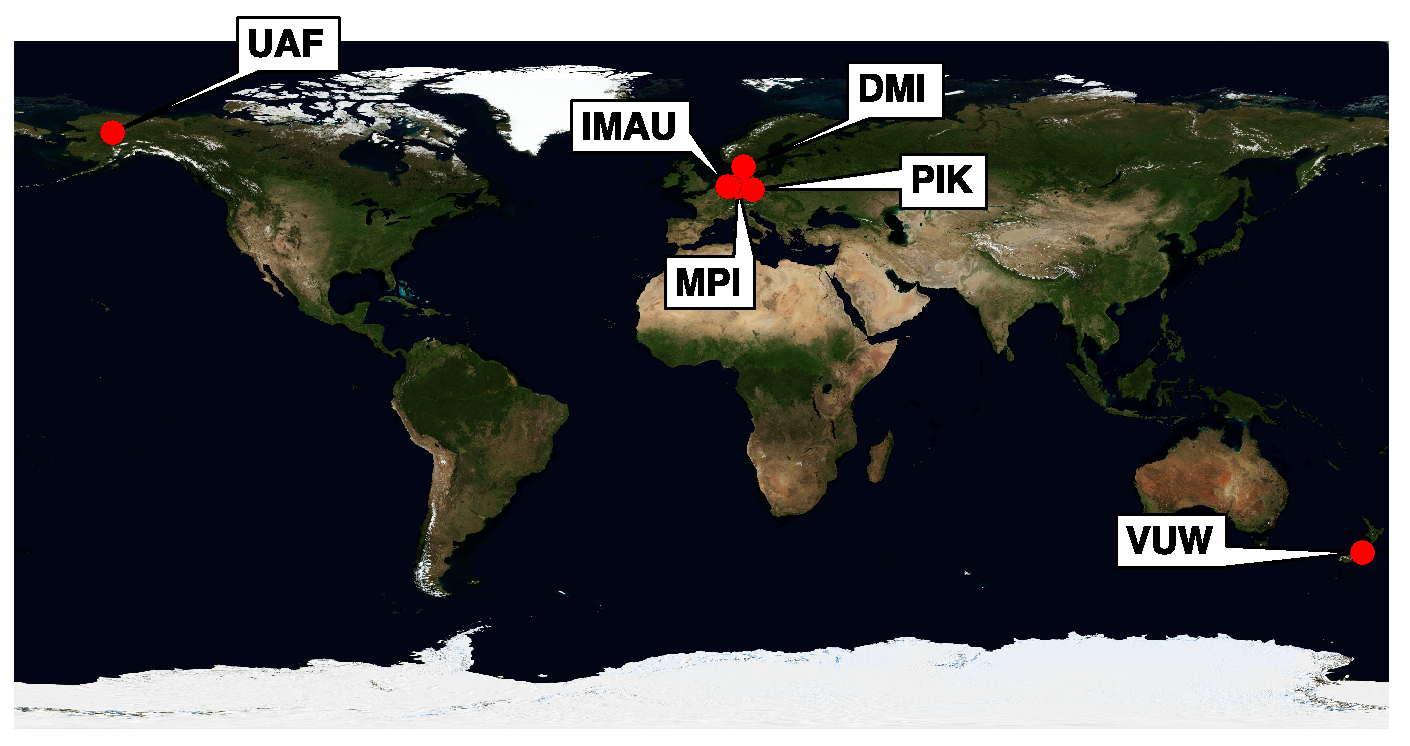
\includegraphics[width=\textwidth]{pism-user-world}
\end{center}
\end{frame}


\section[where's the energy?]{where is the energy in an ice sheet? (and why we care)}\subsection*{}

\begin{frame}
  \frametitle{interjection}

the rest of the talk is joint with 
\begin{itemize}
\item Andy Aschwanden, Arctic Region Supercomputing Center
\item Heinz Blatter, Institute for Atmospheric and Climate Science, ETH Z\"urich
\item Constantine Khroulev, Geophysical Institute
\end{itemize}
\end{frame}


\begin{frame}
  \frametitle{energy in a cubic meter of ice}

  \begin{center}
    % ice cube figure
    \includegraphics[width=0.75\textwidth]{real-ice-cube.jpg}
  \end{center}
\end{frame}


\begin{frame}
  \frametitle{energy in a cubic meter of ice 2}

\begin{itemize}
\item consider a $1\,\text{m}^3$ cube of ice from a glacier
\item mass $m=910$ kg
\item what energies could be associated to this ``glacier cube''?
\end{itemize}

\begin{columns}
\begin{column}{0.25\textwidth}
  \begin{center}
    \includegraphics[width=\textwidth]{cube-drip.jpg}
  \end{center}
\end{column}
\begin{column}{0.85\textwidth}

\begin{itemize}
\item the kinetic energy $\Delta E_{\text{kinetic}}$ to make it move at \emph{fast} glacier speed $v=1000$ meters per year
\item the gravitational potential energy $\Delta E_{\text{potential}}$ it loses in dropping $h=1000$ m
\item the energy $\Delta E_{\text{sensible}}$ needed to heat it by $\Delta T = 10\phantom{|}^\circ\text{C}$
\item the energy $\Delta E_{\text{latent}}$ needed to completely melt it
\end{itemize}
\end{column}
\end{columns}
\end{frame}

\begin{comment}
>> energyscales
energies in Joules:
Ekinetic =  4.5690e-07
Epotential =  8927100
Esensible =  18281900
Elatent =  303940000
\end{comment}


\begin{frame}
  \frametitle{energy scales}

\begin{columns}
\begin{column}{0.2\textwidth}
  \begin{center}
    \includegraphics[width=\textwidth]{cube-drip.jpg}
  \end{center}
\end{column}
\begin{column}{0.85\textwidth}
\begin{align*}
  \Delta E_{\text{kinetic}} &= \frac{1}{2} m v^2 = 4.57 \times 10^{-7} \,\text{J} \\
  &\phantom{=} \\
  \Delta E_{\text{potential}} &= m g h = 8.93 \times 10^{6} \,\text{J} \\
  &\phantom{=} \\
  \Delta E_{\text{sensible}} &= m C \Delta T = 1.83 \times 10^{7} \,\text{J} \\
  &\phantom{=} \\
  \Delta E_{\text{latent}} &= m L = 3.04 \times 10^{7} \,\text{J}
\end{align*}
\end{column}
\end{columns}
\end{frame}


\begin{comment}
>> energyscales
...
energies in Echelmeyers:
Ekinetic =  5.1181e-14
Epotential =  1
Esensible =  2.0479
Elatent =  34.047
\end{comment}

\begin{frame}
  \frametitle{energy scales in natural units}

\emph{Definition}. 

\quad \begin{minipage}[t]{8cm} the energy required to lift a cubic meter of ice by 1000 m in the earth's gravitational field, at sea level, is 1 \emph{Echelmeyer} \quad \small ($= 8.9271 \times 10^6$ J)\normalsize \end{minipage}

\begin{columns}
\begin{column}{0.2\textwidth}
  \begin{center}
    \includegraphics[width=\textwidth]{cube-drip.jpg}
  \end{center}
\end{column}
\begin{column}{0.85\textwidth}
\newcommand{\echel}{\text{\small Echelmeyer}}
\begin{align*}
  \Delta E_{\text{kinetic}} &< 10^{-13} \quad\echel \\
  &\phantom{=} \\
  \Delta E_{\text{potential}} &= 1 \quad\echel \\
  &\phantom{=} \\
  \Delta E_{\text{sensible}} &\approx 2 \quad\echel \\
  &\phantom{=} \\
  \Delta E_{\text{latent}} &\approx 34 \quad\echel
\end{align*}
\end{column}
\end{columns}
\end{frame}


\begin{frame}
  \frametitle{thermodynamics of ice sheets is interesting}

for our cube to go from falling as snow to melting in the ocean, about 2 Echelmeyers must be dissipated:
\begin{itemize}
\small
\item it does not go into kinetic energy (\dots we don't see $100\,\text{m}\,\text{s}^{-1}$ ice in glaciers \dots thank goodness!)
\item the energy does \emph{not} need to stay in the cube
  \begin{itemize}
  \item[$\ast$] internal energy moves from place to place in part by forces (stresses) that do work
  \item[$\ast$] when you in your car drive down the mountain pass, you do lose potential energy but \emph{you} don't heat up \dots just your brakes heat up!
  \end{itemize}
\item it goes into heat somewhere in the glacier, typically
  \begin{itemize}
  \item[$\ast$] near the ice base in thick, fast-flowing ice with high surface slopes
  \end{itemize}
\end{itemize}
\end{frame}


\begin{frame}
  \frametitle{caught my attention!}

when running PISM, I have seen this warning message:
\begin{center}
\scriptsize \texttt{PISM WARNING: fully-liquified cells detected:}

\qquad \texttt{volume liquified = 58.537 km$\hat{\phantom{o}}$3}
\end{center}

\begin{itemize}
\item warning generated because conservation of energy is failing in that part of the modeled fluid \dots
\item this is about 2 trillion Echelmeyers dissipated in one model grid cell in one time step
\item \dots but Greenland volume is $2.93 \times 10^6\,\text{km}^3$, so not much percentage-wise
\item FYI:  typical ice sheet model grid cells are $\approx 10\,\text{km}\times 10\,\text{km} \times 10\,\text{m}$, so volumes $\approx 1\,\text{km}^3$
\item this \texttt{WARNING} happens most often when something \emph{changes} the basal resistance \dots sliding suddenly increases somewhere
\item at the practical level: shortening the time step avoids the warning
\end{itemize}
\end{frame}


\begin{frame}
  \frametitle{Jakobhavn Isbrae \\ = biggest energy dissipator in Greenland}

\begin{columns}
\begin{column}{0.3\textwidth}
\begin{center}
  %\includegraphics[width=\textwidth]{../GGseminar2011/figures/MODISGreenlandJakobshavn}
  \texttt{../GGseminar2011/figures/MODISGreenlandJakobshavn}
\end{center}
\end{column}
\begin{column}{0.7\textwidth}
\begin{center}
  \includegraphics[width=0.7\textwidth]{Joughin2010Fig6_half.png}  
\end{center}
\end{column}
\end{columns}
\end{frame}


\begin{frame}
  \frametitle{borehole temperatures in fast ice: L\"uthi et al (2002)}

\begin{itemize}
\scriptsize
\item note advection bulge
\item at location D, about 33m of temperate ice
\end{itemize}

\vspace{-0.5in}
\begin{center}
  \mbox{\includegraphics[width=0.5\textwidth]{location_luthi2002.png}
\qquad \includegraphics[width=0.5\textwidth]{borehole_temps_luthi2002.png}}
\end{center}
\end{frame}


\begin{frame}
  \frametitle{thought experiment}

consider a drainage basin of Jakobshavn size:
\begin{itemize}
\item 300 km by 300 km $\approx 10^{5}\,\text{km}^2$
\item average rate of added ice by snowfall is 0.2 $\text{m}/\text{yr}$
\item \dots so $V = 20 \,\text{km}^3$ volume of ice is added per year
\item average surface elevation over the basin is about $2000$ m
\item a thought experiment:
\begin{quote}
\emph{In steady state the volume of ice added at the top must equal the volume of ice delivered at sea level.  How much ice can you melt with the dissipated energy?}
\end{quote}
\item i.e.~how much do the brakes heat up?
\end{itemize}
\end{frame}


\begin{frame}
  \frametitle{thought experiment: answer}

\begin{itemize}
\item recall
	$$\frac{\Delta E_{\text{latent}}}{\Delta E_{\text{potential}}} \approx \frac{34\,\text{\small Echelmeyer}}{2\,\text{\small Echelmeyer}} = 17,$$
\item so you can melt about
	$$\frac{20 \,\text{km}^3}{17} \approx 1.2 \,\text{km}^3$$
in one year, if you are adding $V = 20 \,\text{km}^3$ volume of ice per year in the Jakobshavn basin, and it is in steady state
\item an overestimate, because $2\,\text{\small Echelmeyer}$ must be used per $\text{m}^3$ to warm 10 degrees
\item as noted, all this energy is \emph{not} uniformly distributed
  \begin{itemize}
  \item[$\ast$] it appears in places where work rates (= strain rates times deviatoric stresses) are highest
  \item[$\ast$] near the base in thick, fast-flowing ice with high surface slopes
  \end{itemize}
\end{itemize}
\end{frame}


\begin{frame}
  \frametitle{how much ice could be melted in a model time step, Greenland-wide?}
\small

\begin{itemize}
\item if a Greenland-wide surface drop of vertical distance $\Delta z$ occurs in a time step then this much energy is dissipated as heating:
\begin{gather*}
(1.7 \times 10^6\,\text{km}^2) (\Delta z\,\text{m}) (2\,\text{\small Echelmeyer}\,\text{m}^{-3}) \\
  = 3.4 \times 10^{12} \Delta z \,\text{\small Echelmeyer}
\end{gather*}
\item if it all appears as heating near the ice base then this much could melt:
	$$V = 100 \,\Delta z\,\text{km}^3$$
\item this analysis applies if the surface drop is from ice dynamics, but not if it comes from direct atmosphere surface melt
\item compare: $4 \times 10^{11}\,\text{\small Echelmeyer}$ is added by geothermal heat in one year to ice base
\end{itemize}
\end{frame}


\begin{frame}
  \frametitle{role of basal melt}
\small
\begin{itemize}
\item recall this cartoon
  \begin{center}
    \includegraphics[width=0.5\textwidth]{ice-sheet-cartoon}\\
  \end{center}
\item it's true that basal melt \emph{is} a way of losing mass
\item far more interesting, it can \emph{feed back} to the flow, and speed it up
  \begin{itemize}
  \item[$\ast$] this is an instance of ice sheet \emph{dynamics} (= with forces) and not just ice sheet ``mass balance'' (= mere accounting \dots which is hard!)
  \end{itemize}
\end{itemize}
\end{frame}


\begin{frame}
  \frametitle{confounding issue for basal melt: \\ near-basal ice can be partly-melted}
\begin{columns}
\begin{column}{0.6\textwidth}
  \begin{itemize}
  \item near the base of the ice, where there is a high strain-dissipation rate,
  \item \dots and additional geothermal flux and sliding friction,
  \item the ice may not completely melt, but instead build up a liquid fraction of $\omega$, typically of at most a few percent
  \item ice with $\omega > 0$ is \emph{temperate}
  \item we will introduce ``enthalpy'' to deal with this ``polythermal'' issue
  \end{itemize}
\end{column}
\begin{column}{0.4\textwidth}
FIXME: put tempthk-basal figure here; clearly label as ``thickness in meters of temperate ice at the base''
\end{column}
\end{columns}
\end{frame}


\begin{frame}
  \frametitle{should your ice sheet model conserve energy?}

\alert{of course mine does!}  \qquad $\longleftarrow$ \scriptsize say this if funding agency comes calling\normalsize

\bigskip
reasons it should:
\begin{itemize}
\small
\item ice viscosity depends on temperature (and on liquid water content if temperate)
\item basal melt rate is computed from heat fluxes at and near the base of ice, which requires energy balance there
\end{itemize}

\bigskip
it may neglect:
\begin{itemize}
\small
\item kinetic energy
\end{itemize}

\bigskip
we care about basal melt rate because:
\begin{itemize}
\small
\item it dominates subglacial water pressure and thus basal resistance
\item I think it is the critical unknown controlling fast, grounded ice flow in rapidly-changing climates \dots \emph{but I'm just sayin'}
\end{itemize}

\end{frame}


\section[enthalpy]{solid and liquid phases, and enthalpy}\subsection*{}

\begin{frame}
  \frametitle{two kinds of ice: cold and temperate}

\begin{itemize}
\item \emph{cold ice} has temperature below the (pressure-) melting point and no liquid water within the polycrystalline ice matrix\footnote{non-standard usage of ``matrix'', in this building!}
\item \emph{temperate ice} has temperature equal to the melting point and positive amount of liquid water within the matrix
\end{itemize}

\end{frame}


\begin{frame}
  \frametitle{two kinds of thermal structures}

\vspace{-1cm}
  \begin{center}
    \includegraphics[width=0.5\textwidth]{structures}
  \end{center}

\scriptsize two most commonly found polythermal structures (schematic only): a) Canadian-type and b) Scandinavian-type\small

\end{frame}


\begin{frame}
  \frametitle{glacier ice is a mixture of ice and liquid water}

\begin{itemize}
\item mixture density is sum of partial densities:
\begin{equation}
  \rho = \rho_{\text i} +  \rho_{\text w}\notag
\end{equation} 
\item liquid water fraction:
\begin{equation}
  \omega = \frac{\rho_{\text w}}{\rho} \notag
\end{equation}
\item velocity of mixture (``barycentric velocity''):
\begin{equation}
  \rho \mathbf{v} = \rho_{\text i} \mathbf{v}_{\text i} + \rho_{\text w} \mathbf{v}_{\text w} \notag
\end{equation} 
\item because observed $\omega$ are small ($< 3 \%$) we treat the mixture as incompressible:
  $$\rho \approx \hat \rho_{\text i}$$
\end{itemize}
\end{frame}


\begin{frame}
  \frametitle{enthalpy = internal energy}
\small
  
\begin{quote}
Enthalpy is a measure of the total energy of a thermodynamic system.  It includes the internal energy, the energy required to create a system, and the amount of energy required to make room for it by establishing its volume and pressure.\footnote{\tiny Wikipedia, naturally}
\end{quote}
\begin{itemize}
\item that is,
	$$H = U + p V$$
where $H$ is \emph{enthalpy}, $U$ is \emph{internal energy}, $p$ is pressure, and $V$ is the volume of the system
\item but we are applying the enthalpy concept to an incompressible mixture thus the pressure \emph{does no work}
\item so, for our application we may drop $pV$; enthalpy $H$ is an abbreviation for ``internal energy'':
	$$H = U$$
\end{itemize}
\end{frame}


\begin{frame}
  \frametitle{we define enthalpy from temperature and phase}

\begin{itemize}
\item enthalpy for solid ice; $C_{\text i}$ is the specific heat of solid ice:
\begin{equation*}
  H_{\text i}(T) = \int_{T_0}^{T} C_{\text i}(\tilde T)\,\mathrm{d} \tilde T
\end{equation*}
\item enthalpy for liquid water is higher, by at least the latent heat of fusion $L$; $C_{\text w}$ is the specific heat of liquid water:
\begin{equation*}
  H_{\text w}(T,p) = \int_{T_0}^{T_{\text m}(p)} C_{\text i}(\tilde T)\,\mathrm{d} \tilde T + L + \int_{T_{\text m}(p)}^{T} C_{\text w} (\tilde T)\, \mathrm{d} \tilde T,
\end{equation*}
\item here $T_{\text m}(p)$ is the melting temperature, which depends on pressure
\end{itemize}
\end{frame}


\begin{frame}
  \frametitle{enthalpy for the solid/liquid mixture}

\begin{itemize}
\item we define enthalpy for a solid/liquid mixture by the weighted sum:
\begin{equation*}
  \rho H = \rho_{\text i} H_{\text i} + \rho_{\text w} H_{\text w}.
\end{equation*}
\item thus the mixture enthalpy itself is:
\begin{equation*}
   H = H(T,\omega,p) = (1-\omega) H_{\text i}(T) + \omega H_{\text w}(T,p).
\end{equation*}
\item and if the mixture is not completely melted,
\begin{equation*}
 H(T,\omega,p) = \left\{
  \begin{array}{ll} 
    H_{\text i}(T), & \qquad H \le H_{\text s}(p), \\[.25em]
    H_{\text s}(p) + \omega L, & \qquad H_{\text s}(p) < H,
  \end{array}
  \right.
\end{equation*}
where $H_{\text s}(p)$ is the melting-point enthalpy
\end{itemize}
\end{frame}


\begin{frame}
  \frametitle{temperature and liquid fraction are now functions of enthalpy}

\begin{itemize}
\item think: \alert{enthalpy is the basic/state variable}
\item we invert the function $H = H(T,\omega,p)$, giving temperature and liquid fraction as functions of enthalpy and pressure:
\begin{align*}
T(H,p) &= \begin{cases}
          T_{\text i}(H),     & H \le H_{\text s}(p), \\
          T_{\text m}(p),     & H_{\text s}(p) < H,
        \end{cases} \\
\omega(H,p) &= \begin{cases}
          0,                       & H \le H_{\text s}(p), \\
          L^{-1} ( H-H_\text{s}(p) ), & H_{\text s}(p) < H.
        \end{cases}
\end{align*}
\end{itemize}
\end{frame}


\begin{frame}
  \frametitle{diagram explains enthalpy}

\begin{center}
    \input{phase-change.tikz}
\end{center}

\vspace{-0.2in}
\small
\begin{itemize}
\item diagram is for fixed pressure $p$
\item temperature $T$ is solid line
\item liquid water fraction $\omega$ is dotted line
\end{itemize}
\end{frame}


\begin{frame}
  \frametitle{heat flux requires empirical ``constitutive'' relation}
  
\begin{itemize}
\item for cold ice there is Fourier's law, $\mathbf{q} = - k_{\text i} \nabla T$
\item likewise for temperate ice \dots but following the gradient of the pressure-melting temperature
\item \dots thus heat flux is usually upward in cold ice and downward in temperate ice
\item \emph{but} in temperate ice the liquid component may be additionally mobile
\item \emph{empirical relation needed, but few experiments}!
\item we propose a regularized version:
\begin{equation*}
  {\mathbf q} = \left\{
    \begin{array}{rl}
      - k_{\text i} C_{\text i}(H)^{-1}\, \nabla H, & \qquad \text{cold ice},\\
      - k(H,p) \nabla T_{\text m}(p) - k_0 \nabla H, & \qquad \text{temperate ice}.
    \end{array} 
  \right.
\end{equation*}
\item conclusion: conduction in terms of \emph{enthalpy} gradient
\end{itemize}
\end{frame}



\begin{frame}
  \frametitle{summary of the enthalpy concept}

\begin{enumerate}
\item glacier ice is a mixture of ice and liquid water
\item enthalpy may be defined in terms of temperature and liquid water fraction
\item \dots but then temperature and liquid fraction are also functions of enthalpy
\item heat flux in ice requires empirical constitutive relations
\item conduction in terms of \emph{enthalpy} gradient
\end{enumerate}
\end{frame}


\section[jumps and layers]{jumps, thin layers, and the tiniest bit of actual math?}\subsection*{}


\begin{frame}
  \frametitle{mathematics used for ice sheet modeling}
\begin{itemize}
\item continuum mechanics (= calculus for fluids and stuff)
\item + numerical analysis
\item + linear algebra (because you must set up large systems)
\item + scientific computing (because you must \dots compute!)
\end{itemize}

\bigskip\bigskip
\begin{center}
\alert{is there anything new to say in continuum mechanics?}
\end{center}
\end{frame}



\begin{frame}
  \frametitle{review (?) of continuum mechanics}

\begin{itemize}
\item consider a scalar quantity $\psi$ describing particles (fluid) which move with velocity $\mathbf{v}$ within some region $V$
  \begin{itemize}
  \item[$\ast$] e.g.~enthalpy or density
  \end{itemize}
\item the \emph{advective flux} is $\psi \mathbf{v}$
\item there may be additional \emph{non-advective} flux $\boldsymbol{\phi}$
  \begin{itemize}
  \item[$\ast$] e.g.~conductive/diffusive flux
  \end{itemize}
\item there may be \emph{production} of $\psi$ at rate $\pi$
\item then the \alert{general balance eqn} for $\psi$ is:
\begin{equation*}
  \frac{\partial \psi}{\partial t} = - \nabla \cdot \left(\psi \mathbf{v} + \boldsymbol{\phi} \right) + \pi
\end{equation*}
\item this is an Eulerian view of the fluid, as the region $V$ is fixed
\end{itemize}
\end{frame}


\begin{frame}
  \frametitle{example: mixture enthalpy balance}

\begin{itemize}
\item we formulate separate component energy balances for $\psi=\rho_{\text i} H_{\text i}$ and $\psi = \rho_{\text w} H_{\text w}$:
\scriptsize
\begin{align*}
  \frac{\partial (\rho_{\text i} H_{\text i})}{\partial t} &= - \nabla \cdot \left(\rho_{\text i} H_{\text i} \bv + \mathbf{q}_{\text i}\right) + Q_{\text i} - \Sigma_{\text w} \\
  \frac{\partial (\rho_{\text w} H_{\text w})}{\partial t} &= - \nabla \cdot \left(\rho_{\text w} H_{\text w} \bv + \mathbf{q}_{\text w}\right) + Q_{\text w} + \Sigma_{\text w}
\end{align*}
\normalsize
\item $\Sigma_{\text i},\Sigma_{\text w}$ are energy \emph{exchange} rates between components
\item conservation of energy in small pieces of mixture: $\Sigma_{\text i}+\Sigma_{\text w}=0$
\item adding and simplifying, along with mass conservation, gives a mixture balance, the \alert{conservation of energy equation}
    $$\rho \frac{\text{d} H}{\text{d}t}  = - \nabla \cdot \mathbf{q} + Q$$
\end{itemize}
\end{frame}


\begin{frame}
  \frametitle{review of continuum mechanics 2}

\begin{itemize}
\item suppose some scalar quantity $\psi$ satisfies a general balance eqn
\item consider a region $V$ split by a surface $\sigma$, in which $\psi$ is discontinuous across $\sigma$
\item $\sigma$ has normal vector $\mathbf{n}$; might move with normal speed $w$
  \begin{itemize}
  \item[$\ast$] we assume $\psi$ has limits as you approach $\sigma$
  \item[$\ast$] we assume boundedness on $\partial\psi/\partial t$ and $\pi$
  \end{itemize}
\item apply a ``pillbox'' (shown below) argument
\end{itemize}

  \begin{center}
    \includegraphics[width=0.6\textwidth]{simplepillbox}
  \end{center}
\end{frame}


\begin{frame}
  \frametitle{review of continuum mechanics 3}

\begin{itemize}
\item the integral form of the general balance them implies a \alert{jump equation}
	$$\jl \psi (\mathbf{v} \cdot \mathbf{n} - w) \jr + \jl \boldsymbol{\phi} \cdot \mathbf{n} \jr =0$$
where
	$$\jl f \jr = f^+ - f^-$$
\item jump eqn also called \emph{Rankine-Hugoniot equation}
\end{itemize}

  \begin{center}
    \includegraphics[width=0.6\textwidth]{simplepillbox}
  \end{center}
\end{frame}


\begin{frame}
  \frametitle{mixture fields defined even outside of ice sheet}
\begin{itemize}
\item consider scalar $\rho H$= (ice/water mixture enthalpy density)
\item it is defined in air, ice, and bedrock
  \begin{itemize}
  \item[$\ast$] but it is zero outside of ice (dry air and dry rock assumptions)
  \end{itemize}
\item it jumps at the ice upper surface and the ice base
\end{itemize}

\begin{center}
\resizebox{0.7\textwidth}{!}{
        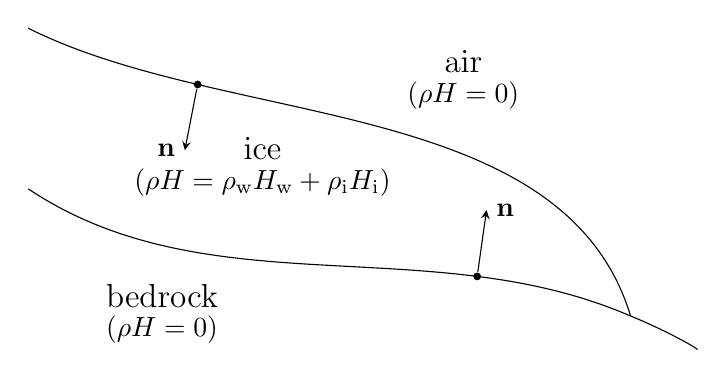
\begin{tikzpicture}[>=stealth,scale=1.7]
      \draw (-2,1) .. controls (-.5,.25) and (2,.5) .. (2.5,-1.15) node[pos=0.25,inner sep=1pt,circle,fill] (iceair) {}; % ice surface
      \draw (-2,-.2) .. controls (-.65,-1.1) and (1,-.5) .. (2.5,-1.15) node[pos=0.75,inner sep=1pt,circle,fill] (icebedrock) {}; % bedrock
      \draw (2.5,-1.15) .. controls (2.7,-1.23) and (2.95,-1.36) .. (3,-1.4); % bedrock extension
      \node (air1) at (1.25,0.75) {{\large air}};
      \node (air2) at (1.25,0.50) {($\rho H = 0$)};
      \node (ice1) at (-.25,0.10) {{\large ice} };
      \node (ice2) at (-.25,-0.15) {($\rho H = \rho_{\text w} H_{\text w} + \rho_{\text i} H_{\text i}$)};
      \node (bedrock1) at (-1,-1) {{\large bedrock}};
      \node (bedrock2) at (-1,-1.25) {($\rho H = 0$)};
     \draw[->] (iceair) -- +(-101:.5cm) node[anchor=east] {$\bf{n}$};
     \draw[->] (icebedrock) -- +(82:.5cm) node[anchor=west] {$\bf{n}$};
  \end{tikzpicture}

}
\end{center}
\end{frame}



\begin{frame}
  \frametitle{jump conditions across thin-layer transport}
\small

\begin{itemize}
\item consider a thin subglacial hydrologic layer  $V^0$ at base of ice sheet in which liquid can flow fast ($O(1)$ m/s)
\item surfaces $\Sigma^\pm$ bound the layer
\item need to modify the pillbox argument
  \begin{itemize}
  \item[$\ast$] take the $\delta^0 \to 0$ limit of a thin transport layer concentrated into the surface $\sigma$
  \item[$\ast$] surfaces $\Sigma^\pm$ converge to a single surface $\sigma$
  \end{itemize}
\item standard jump eqns ($\jl \psi (\mathbf{v} \cdot \mathbf{n} - w) \jr + \jl \boldsymbol{\phi} \cdot \mathbf{n} \jr =0$) apply on  $\Sigma^\pm$
\end{itemize}

  \begin{center}
    \includegraphics[width=0.6\textwidth]{pillbox}
  \end{center}
\end{frame}


\begin{frame}
  \frametitle{jump conditions across thin-layer transport 2}

\begin{itemize}
\item the result is \emph{both} a jump equation and a thin-layer balance:
\begin{equation*}
\jl \psi (\mathbf{v} \cdot \mathbf{n} - w) \jr + \jl \boldsymbol{\phi} \cdot \mathbf{n} \jr + \frac{\partial \lambda_\sigma}{\partial t} + \nabla \cdot\left(\lambda_\sigma \bv_\sigma + \bphi_\sigma\right) = \pi_\sigma.
\end{equation*}
where these quantities are only defined in the surface $\sigma$:
  \begin{itemize}
  \item[$\ast$] $\lambda_\sigma$ is area density of quantity $\psi$
  \item[$\ast$] $\mathbf{v}_\sigma$ is velocity in the thin-layer
  \item[$\ast$] $\bphi_\sigma$, $\pi_\sigma$ are non-advective flux and production, resp.
  \end{itemize}
\item this jump equation is specialized \dots and maybe new
\end{itemize}
\end{frame}


\begin{frame}
  \frametitle{basal melt rate}

\begin{itemize}
\item again consider $\psi=\rho H$ the mixture enthalpy density $\rho H$
\item how does it jump at the ice base?
\item identify the rate at which the thin-subglacial layer can transport enthalpy to a location on the ice base as $Q_b$; this must be modeled by understanding actual physics of such subglacial layers!
\item let $F_b = \bv \cdot (\mathbf{T}\cdot \mathbf{n})$= (rate of friction heating from sliding)
\item then the jump-equation-and-thin-layer-balance is:
\begin{equation*}
M_b H + \left(\bq - \bq_{\text{lith}}\right)\cdot \bn \stackrel{\dagger}{=} F_b + Q_b
\end{equation*}
where $\bq,\bq_{\text{lith}}$ are conductive heat fluxes in ice and bedrock respectively
\item equation $(\dagger)$ \alert{computes the basal melt rate} $M_b$ from more complete conservation than before (maybe new \dots)
\end{itemize}
\end{frame}


\begin{frame}
  \frametitle{PISM-modeled basal melt rate}

\begin{columns}
\begin{column}{0.6\textwidth}
\begin{itemize}
\item suppose you put that stuff in your model:
  \begin{itemize}
  \item[$\ast$] eqns of ice flow: stress balance, mass conservation
  \item[$\ast$] conservation of energy using enthalpy
  \item[$\ast$] new basal melt rate eqn
  \end{itemize}
\item model might give basal melt rate (m/year) at right
\item \emph{is it correct?}
\item basal melt rate may be important to dynamics, \emph{but it is very hard to observe}
\end{itemize}
\end{column}
\begin{column}{0.4\textwidth}
\begin{center}
    \includegraphics[width=\textwidth]{bmelt_result}
  \end{center}
\end{column}
\end{columns}
\end{frame}


\begin{frame}
  \frametitle{PISM-modeled thermodynamics}

\begin{columns}
\begin{column}{0.5\textwidth}
\begin{itemize}
\small
\item important diagnostic: \emph{proportion of the ice sheet that is temperate}
\item figure at right shows fraction of Greenland area which has some temperate ice
\item shows instability, despite model using steady boundary conditions
\item \emph{is this instability real?}
\end{itemize}
\end{column}
\begin{column}{0.5\textwidth}
\begin{center}
    \includegraphics[width=\textwidth]{10kmfine_iareatempf}
  \end{center}
\end{column}
\end{columns}
\end{frame}


\begin{frame}
  \frametitle{PISM-modeled thermodynamics 2}

\begin{columns}
\begin{column}{0.6\textwidth}
\begin{itemize}
\small
\item important diagnostic: \emph{thickness of temperate layer}
\item recall L\"uthi et al (2002) borehole measurements
  \begin{itemize}
  \item[$\ast$] borehole D had 33 m of temperate ice
  \item[$\ast$] we get 51 m in this run
  \end{itemize}
\item lacking more than a few validating measurements
\item but the purpose of a model is to help you see what you can't see!
\item \alert{THE END.}  Did I help with your ice sheet modeling problems?
\end{itemize}
\end{column}
\begin{column}{0.4\textwidth}
\begin{center}
    \includegraphics[width=\textwidth]{bmelt_result_boreD}
  \end{center}
\end{column}
\end{columns}
\end{frame}


\end{document}

